\documentclass[12pt]{article}
\usepackage{setspace,graphicx,amsmath,geometry,fontspec,titlesec,soul,bm,subfigure}
\titleformat{\section}[block]{\LARGE\bfseries}{\arabic{section}}{1em}{}[]
\titleformat{\subsection}[block]{\Large\bfseries\mdseries}{\arabic{section}.\arabic{subsection}}{1em}{}[]
\titleformat{\subsubsection}[block]{\normalsize\bfseries}{\arabic{subsection}-\alph{subsubsection}}{1em}{}[]
\titleformat{\paragraph}[block]{\small\bfseries}{[\arabic{paragraph}]}{1em}{}[]
\setmainfont{Times New Roman}
\renewcommand{\baselinestretch}{1.15}
\renewcommand\contentsname{Inhaltverzeichnis}
\geometry{a4paper,left=2.5cm,right=2.5cm,top=2.5cm,bottom=2.5cm}
\begin{document}
	\newpagestyle{main}{            
		\sethead{Ziqing Yu}{Physikalische Geodäsie Übung 4}{3218051}     
		\setfoot{}{\thepage}{}     
		\headrule                                     
		\footrule                                       
	}
	\pagestyle{main}
\tableofcontents
\newpage
\section{Gravity, gravitation and centrifugal acceleration}
\subsection{}
Die Dichte von Erde ist $\rho = 5515 kg/m^3$, der Radius ist $R = 6371 km$, und die Winkelgeschwindigkeit ist $\omega = 7.292115 \cdot 10^{-5} s^{-1}$. Der Punkt ist auf der Erdebene, das bedeutet, $r = R = 6371 km$. Die Länge bzw. Breite sind $10°$ bzw. $22°$ (mit k = 1). 
\newline
Die Gravitation Potential:
\begin{equation*}
V = \frac{4}{3} \pi G \rho R^3 \frac{1}{r} = 6,2561 \cdot 10^7 m^2/s^2
\end{equation*}
Die Zentrifugal Potential:
\begin{equation*}
V_c = \frac{1}{2} \omega^2 r^2 \cos^2(\phi) = 9,2774 \cdot 10^4 m^2/s^2
\end{equation*}
Die Gravitation Anziehung
\begin{equation*}
\bm{a} = - \frac{4}{3} \frac{1}{r^3} \pi G \rho R^3  \begin{bmatrix} x\\ y\\ z \end{bmatrix},\quad mit \begin{bmatrix} x\\ y\\ z \end{bmatrix} = \begin{bmatrix} r \cos(\phi) \cos(\lambda) \\ \r \cos(\phi) \sin(\lambda)\\ r \sin(\phi) \end{bmatrix}
\end{equation*}
\begin{equation*}
a =|\bm{a}| = 9,8197 m/s^2
\end{equation*}
Die Schwerbeschleunigung $g$
\begin{equation*}
\bm{a_c} = \omega^2 \begin{bmatrix} x\\ y\\ 0 \end{bmatrix}
\end{equation*}
\begin{equation*}
\bm{g} = \bm{a} + \bm{a_c}
\end{equation*}
\begin{equation*}
g = |\bm{g}| = 9,7906 m/s^2
\end{equation*}
Die Störung von Richtung
\begin{equation*}
\xi = \arccos(\frac{\bm{a} \cdot \bm{g}}{|\bm{a}| |\bm{g}|}) = 0,0689°
\end{equation*}
Die Störung von Betrag
\begin{equation*}
\sigma_g = g - a = -0,0291 m/s^2
\end{equation*}
\newpage
\subsection{}
Die Störung in Richtung bzw. Betrag und Zentrifugal Potential innerhalb $0°$ bis $90°$
\begin{figure}[ht]\centering
	\subfigure[Störung in Richtung $\xi$]{
		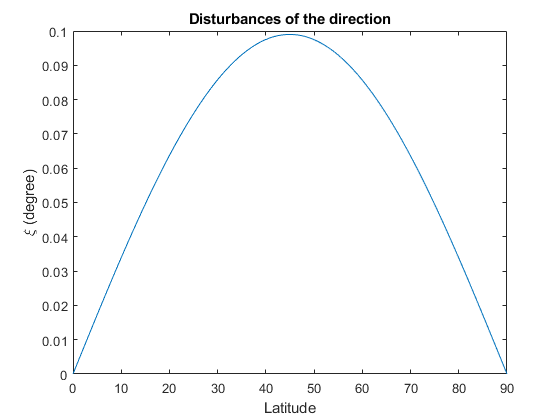
\includegraphics[width=0.45\textwidth]{direction.png}}
	\subfigure[Störung in Betrag $\sigma _g$]{
		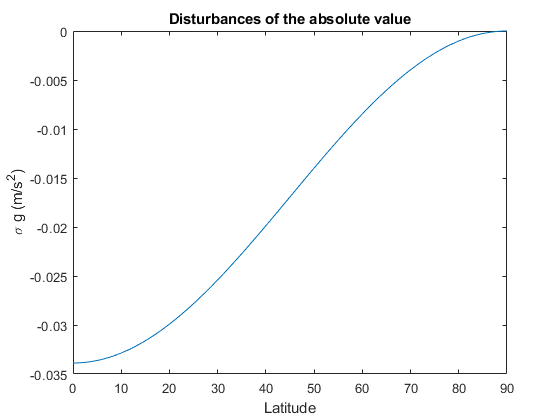
\includegraphics[width=0.45\textwidth]{value.png}}
	\subfigure[Zentrifugal Potential $V_c$]{
		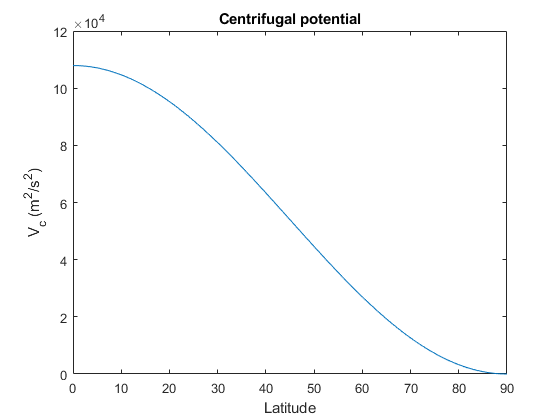
\includegraphics[width=0.45\textwidth]{centrifugal.png}}
	\caption{Darstellung}
\end{figure}
\newpage
\section{Eötvös correction}
In dieser Aufgabe ist Eötvös Korrektur zu berechnen. Die Geschwindigkeit der Flugzeug ist $400km/h$ also $111,11m/s$. Die Breite $\phi = 42°$. Um die Rechnungen einfacher zu sein, nennen wir $\theta = 90° - \phi = 48°$.
\newline
\newline
Weil die Geschwindigkeiten gleich in beiden Richtungen sind 
\begin{equation*}
v_{EW} = v_{NS} = \frac{v}{\sqrt{2}} = 78,57 m/s
\end{equation*}
Coriolis Beschleunigung in Ost-West Richtung:
\begin{equation*}
a^{EW}_{cor} = 2 \omega \begin{bmatrix} - \cos (\theta) v_{EW}\\ 0\\ \sin (\theta) v_{EW} \end{bmatrix}
= \begin{bmatrix} -0,0077\\ 0\\ 0,0085 \end{bmatrix} m/s^2
\end{equation*}
Coriolis Beschleunigung in Nord-Süd Richtung
\begin{equation*}
a^{NS}_{cor} = 2 \omega \begin{bmatrix} 0\\ \cos (\theta) v_{NS}\\ 0 \end{bmatrix} = \begin{bmatrix} 0\\ 0,0077\\ 0 \end{bmatrix} m/s^2
\end{equation*}
Die Eötvös Korrektur ist nur in $z$ Richtung, das bedeutet, $E_{EW} = -0,0085 m/s^2$ und $E_{NS} = 0$
\newline
\newline
Die Eötvös Korrektur ist nur von die Geschwindigkeit in Ost-West Richtung abhängig. Wenn wir die Genauigkeit von Eötvös Korrektur 1mGal brauchen: 
\begin{equation*}
\sigma_E = 1mGal = 10^{-5} m/s^2
\end{equation*}
\begin{equation*}
\sigma_{v_{EW}} = \frac{\sigma_E}{2 \omega \sin(\theta)} = 0,0923 m/s
\end{equation*}
Die Genauigkeit von Ost-West Geschwindigkeit muss $0,0923 m/s$ sein.
\end{document}